\cleardoublepageeven
\section{cumulative}
\hypertarget{Ccumulative}{}
\sbox{\signbox}{\small$\overline{\graphproperty{NARC}},\arcgenerator{SELF};\arcgenerator{PRODUCT},\setgenerator{SUCC}$}
\index{signature!NARCSELFPRODUCTSUCC@\small$\overline{\graphproperty{NARC}},\arcgenerator{SELF};\arcgenerator{PRODUCT},\setgenerator{SUCC}$!cumulative@$\constraint{cumulative}$|indexuse}
\markboth{\usebox{\signbox}}{20000128}
\def\Morigin{\argument{origin}}
\def\Mduration{\argument{duration}}
\def\Mend{\argument{end}}
\def\MTASKS{\argument{TASKS}}
\def\MLIMIT{\argument{LIMIT}}
\def\MNARC{\graphproperty{NARC}}
\def\examplefig{}
\def\examplefigv{}
\begin{tabular}{l@{\hspace{.15\textwidth}}l@{\hspace{.15\textwidth}}l@{\hspace{.15\textwidth}}l}
\bf \hyperlink{CcumulativePdesc}{DESCRIPTION} & \bf \hyperlink{CcumulativePlinks}{LINKS} & \bf \hyperlink{CcumulativePgraph}{GRAPH} & \bf \hyperlink{CcumulativePauto}{AUTOMATON} \\
\end{tabular}
\begin{ctrdesc}
\index{Aggoun A.|indexuse}
\index{Baptiste P.|indexuse}
\index{Beldiceanu N.|indexuse}
\index{Caseau Y.|indexuse}
\index{Demassey S.|indexuse}
\index{Erschler J.|indexuse}
\index{Hooker J. N.|indexuse}
\index{Laburthe F.|indexuse}
\index{Lahrichi A.|indexuse}
\index{Le Pape C.|indexuse}
\index{Lock H. C. R.|indexuse}
\index{Lopez P.|indexuse}
\index{Yan H.|indexuse}
\index{Carlsson M.|indexuse}
\index{Poder E.|indexuse}
\index{Mercier L.|indexuse}
\index{Van Hentenryck P.|indexuse}
\index{Vil\'im P.|indexuse}
\index{Schutt A.|indexuse}
\index{Wolf A.|indexuse}
\index{Kameugne R.|indexuse}
\index{Fotso L. P.|indexuse}
\index{Scott J.|indexuse}
\index{Ngo-Kateu Y.|indexuse}
\index{cumulative@$\constraint{cumulative}$|indexdef}
\item[\pdfmarkup{subject={Origin},color=white,markup=Highlight}{Origin}{The origin of the constraint: reference to a paper, to a person, to an other constraint or to a system.}]
\hypertarget{CcumulativePdesc}{}
\cite{AggounBeldiceanu93}
\item[\pdfmarkup{subject={Constraint},color=white,markup=Highlight}{Constraint}{The constraint name and its arguments.}]
\colorbox{MyAzurelight}{\begin{minipage}[t]{11.2cm}
$\constraint{cumulative}(\argument{TASKS},\argument{LIMIT})$
\end{minipage}}
\item[\pdfmarkup{subject={Synonym},color=white,markup=Highlight}{Synonym}{A synonym for the name of the constraint.}]
\colorbox{MyAzurelight}{\begin{minipage}[t]{11.2cm}
$\constraint{cumulative\_max}$.\hfill
\index{cumulative\_max@$\constraint{cumulative\_max}$|indexsyn}

\end{minipage}}
\item[\pdfmarkup{subject={Arguments},color=white,markup=Highlight}{Arguments}{Arguments of the constraint and their corresponding types.}]
\colorbox{MyAzurelight}{\begin{minipage}[t]{11.2cm}
\begin{tabular}[t]{l@{\quad:\quad}l}
$\argument{TASKS}$ & $ $\hyperlink{DT_collection}{$\argument{collection}$}$ \left(\begin{array}{l}
\argument{origin}- $\hyperlink{DT_dvar}{$\argument{dvar}$}$ ,
\\\argument{duration}- $\hyperlink{DT_dvar}{$\argument{dvar}$}$ ,
\\\argument{end}- $\hyperlink{DT_dvar}{$\argument{dvar}$}$ ,
\\\argument{height}- $\hyperlink{DT_dvar}{$\argument{dvar}$}$ \\
\end{array}\right) $ \\
$\argument{LIMIT}$ & $ $\hyperlink{DT_int}{$\argument{int}$}$ $ \\
\end{tabular}

\end{minipage}}
\item[\pdfmarkup{subject={Restrictions},color=white,markup=Highlight}{Restrictions}{Additional conditions refining the type declarations of one or several arguments of the constraint.}]
\colorbox{MyAzurelight}{\begin{minipage}[t]{11.2cm}
\begin{tabular}[t]{l}
$ $\hyperlink{PR_require_at_least}{$\argument{require\_at\_least}$}$ (2,\argument{TASKS},\lb\argument{origin},\argument{duration},\argument{end}\rb)$\\
$ $\hyperlink{PR_required}{$\argument{required}$}$ (\argument{TASKS},\argument{height})$\\
$\argument{TASKS}.\argument{duration}\geq 0$\\
$\argument{TASKS}.\argument{origin}\leq \argument{TASKS}.\argument{end}$\\
$\argument{TASKS}.\argument{height}\geq 0$\\
$\argument{LIMIT}\geq 0$\\
\end{tabular}

\end{minipage}}
\item[\pdfmarkup{subject={Purpose},color=white,markup=Highlight}{Purpose}{Definition in natural language of the meaning of the constraint.}]
{\setlength\fboxrule{1.5pt}\fcolorbox{MyRed}{white}{\begin{minipage}{11.1cm}
Cumulative scheduling constraint or scheduling under resource
constraints. Consider a set $\mathcal{T}$ of tasks described by
the $\MTASKS$ collection. The \ctrrefself{cumulative} constraint
enforces that at each point in time, the cumulated height of the
set of tasks that overlap that point, does not exceed a given limit.
A task overlaps a point $i$ if and only if
(1)~its origin is less than or equal to $i$, and
(2)~its end is strictly greater than $i$.
It also imposes for each task of $\mathcal{T}$ the constraint
$\Morigin+\Mduration=\Mend$.

\end{minipage}}}
\medskip
\def\examplefig{\examplefigiih{fig:cumulative}{Initial and final graph of the \ctrrefself{cumulative} constraint}{ctrs/cumulativeA}{ctrs/cumulativeB}}
\def\examplefigv{\examplefigiiv{fig:cumulative}{Initial and final graph of the \ctrrefself{cumulative} constraint}{ctrs/cumulativeA}{ctrs/cumulativeB}}
\item[\pdfmarkup{subject={Example},color=white,markup=Highlight}{Example}{One or several examples of ground solutions of the constraint.}]
{\setlength\fboxrule{1.5pt}\fcolorbox{MyCornflowerBlue}{MyYellowlight}{\makebox[\width]{
\begin{tabular}[t]{l}
$\argument{}\left(\begin{array}{l}
\left\langle\begin{array}{llll}
\argument{origin}-1&\argument{duration}-3&\argument{end}-4&\argument{height}-1,\\
\argument{origin}-2&\argument{duration}-9&\argument{end}-11&\argument{height}-2,\\
\argument{origin}-3&\argument{duration}-10&\argument{end}-13&\argument{height}-1,\\
\argument{origin}-6&\argument{duration}-6&\argument{end}-12&\argument{height}-1,\\
\argument{origin}-7&\argument{duration}-2&\argument{end}-9&\argument{height}-3\\
\end{array}\right\rangle ,
8\\
\end{array}\right) $\\
\end{tabular}

}}}
\\\ \\
\begin{figure}[!h]
\centering
\begin{tikzpicture}[information text/.style={rounded corners,inner sep=1ex}]
\begin{scope}[scale=0.5]
\draw[step=1cm,gray,very thin] (0,0) grid (13,8);
\filldraw[fill=yellow, draw=black!65, line width=0.6pt] (1,0) rectangle (2,1);
\filldraw[fill=black, draw=black] (1,0) rectangle (1.25,0.25);
\coordinate [label=left:\textcolor{black}{{\bf\ding{172}}}] (T1) at (2,0.5);
\filldraw[fill=yellow, draw=black!65, line width=0.6pt] (2,2) rectangle (3,3);
\coordinate [label=left:\textcolor{black}{{\ding{172}}}] (T1) at (3,2.5);
\filldraw[fill=yellow, draw=black!65, line width=0.6pt] (3,3) rectangle (4,4);
\coordinate [label=left:\textcolor{black}{{\ding{172}}}] (T1) at (4,3.5);
\filldraw[fill=pink, draw=black!65, line width=0.6pt] (2,0) rectangle (11,2);
\filldraw[fill=black, draw=black] (2,0) rectangle (2.25,0.25);
\coordinate [label=left:\textcolor{black}{{\bf\ding{173}}}] (T1) at (6.95,1.0);
\filldraw[fill=MyLightBlue, draw=black!65, line width=0.6pt] (3,2) rectangle (11,3);
\filldraw[fill=black, draw=black] (3,2) rectangle (3.25,2.25);
\coordinate [label=left:\textcolor{black}{{\bf\ding{174}}}] (T1) at (6.95,2.5);
\filldraw[fill=MyLightBlue, draw=black!65, line width=0.6pt] (11,0) rectangle (13,1);
\coordinate [label=left:\textcolor{black}{{\ding{174}}}] (T1) at (12.5,0.55);
\filldraw[fill=green!50, draw=black!65, line width=0.6pt] (6,3) rectangle (11,4);
\filldraw[fill=black, draw=black] (6,3) rectangle (6.25,3.25);
\coordinate [label=left:\textcolor{black}{{\bf\ding{175}}}] (T1) at (8.95,3.5);
\filldraw[fill=green!50, draw=black!65, line width=0.6pt] (11,1) rectangle (12,2);
\coordinate [label=left:\textcolor{black}{{\ding{175}}}] (T1) at (12,1.5);
\filldraw[fill=red!50, draw=black!65, line width=0.6pt] (7,4) rectangle (9,7);
\filldraw[fill=black, draw=black] (7.05,4) rectangle (7.3,4.25);
\coordinate [label=left:\textcolor{black}{{\bf\ding{176}}}] (T1) at (8.5,5.5);
\foreach \x in {1,2,3,4,5,6,7,8,9,10,11,12,13}
\draw[draw=black,line width=0.5pt] (\x,0) -- (\x,0.2);
\draw[draw=black,line width=0.8pt,->] (0,0) -- (14.25,0);
\foreach \x in {1,2,3,4,5,6,7,8,9,10,11,12,13}
\coordinate [label=left:{\scriptsize$\x$}] (X) at (0.5+\x,-0.5);
\foreach \y in {1,2,3,4,5,6,7,8}
\draw[draw=black,line width=0.5pt] (0,\y) -- (0.2,\y);
\foreach \y in {1,2,3,4,5,6,7,8}
\coordinate [label=left:{\scriptsize$\y$}] (Y) at (-0.1,\y+0.1);
\draw[draw=red,line width=2.0pt] (0,8) -- (13,8);
\draw[draw=black,line width=0.8pt,->] (0,0) -- (0,8.75);
\draw[draw=red!90,line width=2.0pt,rounded corners=2pt] (0.95,0) -- (0.95,1) -- (2,1) -- (2,3) -- (3,3) -- (3,4) -- (4,4) -- (4,3) -- (5.95,3) -- (5.95,4)  -- (6.95,4) -- (6.95,7) -- (9,7) -- (9,4) -- (11,4) -- (11,2) -- (12,2) -- (12,1) -- (13,1) -- (13,0);
\coordinate [label=left:{\color{red}{\scriptsize $\leq 8$}}] (L) at (14.5cm,8.0cm);
\coordinate [label=left:{\color{black}{\footnotesize time}}] (L) at (15.2cm,-0.6cm);
\node[rotate=90] at (-1.2,6.0) {{\footnotesize amount of used resource}};
\end{scope}
\begin{scope}[xshift=0.5cm,yshift=6.8cm]
\node[right,information text,fill=MyYellowlight,draw=MyCornflowerBlue,line width=1.5pt] (tasks)
{\footnotesize
\begin{tabular}{lllll}
\ding{172}&$\argument{o}-1$&$\argument{d}-3$&$\argument{e}-4$&$\argument{h}-1$\\
\ding{173}&$\argument{o}-2$&$\argument{d}-9$&$\argument{e}-11$&$\argument{h}-2$\\
\ding{174}&$\argument{o}-3$&$\argument{d}-10$&$\argument{e}-13$&$\argument{h}-1$\\
\ding{175}&$\argument{o}-6$&$\argument{d}-6$&$\argument{e}-12$&$\argument{h}-1$\\
\ding{176}&$\argument{o}-7$&$\argument{d}-2$&$\argument{e}-9$&$\argument{h}-3$
\end{tabular}};
\draw (tasks.north west) node [anchor=south west] {\small$\argument{TASKS}$};
\draw (tasks.south west) node [anchor=north west] {\footnotesize$\left(\begin{array}{ll}
\argument{o}\text{ for }\argument{origin}\text{,} & \argument{d}\text{ for }\argument{duration}\text{,}\\
\argument{e}\text{ for }\argument{end}\text{,} & \argument{h}\text{ for }\argument{height}
\end{array}\right)$};
\end{scope}
\end{tikzpicture}
\caption{\label{fig:cumulative1}
Resource consumption profile corresponding to the five tasks of the {\bf Example} slot
(note that the vertical position of a task does not really matter but is only used
for displaying the contribution of a task to the resource consumption profile)}
\end{figure}

Figure~\ref{fig:cumulative1} shows the cumulated profile associated with the example.
To each task of the \ctrrefself{cumulative} constraint, i.e.~each line of the example,
corresponds a set of rectangles coloured with the same colour: the sum of the lengths
of the rectangles corresponds to the duration of the task, while the height of the rectangles
(i.e., all the rectangles associated with a task have the same height) corresponds to the
resource consumption of the task. The \ctrrefself{cumulative} constraint holds since at
each point in time we do not have a cumulated resource consumption strictly greater
than the upper limit $8$ enforced by the last argument of the \ctrrefself{cumulative}
constraint.

\ifweb\else
\newpage
\fi
\item[\pdfmarkup{subject={All solutions},color=white,markup=Highlight}{All solutions}{Example of all solutions for a non ground instance of the constraint.}]
Figure~\ref{fig:cumulative0} gives all solutions to the following non ground instance of the \ctrrefself{cumulative} constraint:\\
$O_1\in [1,5]$, $D_1\in [4,4]$, $E_1\in [1,9]$, $H_1\in [2,6]$,\\
$O_2\in [2,7]$, $D_2\in [6,6]$, $E_2\in [1,9]$, $H_2\in [3,3]$,\\
$O_3\in [3,6]$, $D_3\in [3,6]$, $E_3\in [1,9]$, $H_3\in [1,2]$,\\
$O_4\in [1,8]$, $D_4\in [2,3]$, $E_4\in [1,9]$, $H_4\in [3,4]$,\\
\ctrrefself{cumulative}$(\langle 	O_1~D_1~E_1~H_1~1,~
O_2~D_2~E_2~H_2~2,~
O_3~D_3~E_3~H_3~3,~
O_4~D_4~E_4~H_4~4 \rangle,5)$.
\begin{figure}[!h]
\centering
{\small
\begin{tikzpicture}
\begin{scope}[every node/.style={single arrow, single arrow tip angle=135, single arrow head extend=1cm, draw=MyCornflowerBlue, line width=2pt}]
\node [fill=MyYellowlight, single arrow, shape border rotate=270, text width=6.3 cm]
{\ding{172} $(\langle	{\color{MyRhodamine}\mathbf{1~4~5~2}},~~
{\color{MyRedOrange}\mathbf{3~6~9~3}},~~
{\color{MyPineGreen}\mathbf{5~3~8~1}},~~
{\color{MyCornflowerBlue}\mathbf{1~2~3~3}}\rangle)$\\
\ding{173} $(\langle	{\color{MyRhodamine}\mathbf{1~4~5~2}},~~
{\color{MyRedOrange}\mathbf{3~6~9~3}},~~
{\color{MyPineGreen}\mathbf{5~3~8~2}},~~
{\color{MyCornflowerBlue}\mathbf{1~2~3~3}}\rangle)$\\
\ding{174} $(\langle	{\color{MyRhodamine}\mathbf{1~4~5~2}},~~
{\color{MyRedOrange}\mathbf{3~6~9~3}},~~
{\color{MyPineGreen}\mathbf{5~4~9~1}},~~
{\color{MyCornflowerBlue}\mathbf{1~2~3~3}}\rangle)$\\
\ding{175} $(\langle	{\color{MyRhodamine}\mathbf{1~4~5~2}},~~
{\color{MyRedOrange}\mathbf{3~6~9~3}},~~
{\color{MyPineGreen}\mathbf{5~4~9~2}},~~
{\color{MyCornflowerBlue}\mathbf{1~2~3~3}}\rangle)$\\
\ding{176} $(\langle	{\color{MyRhodamine}\mathbf{1~4~5~2}},~~
{\color{MyRedOrange}\mathbf{3~6~9~3}},~~
{\color{MyPineGreen}\mathbf{6~3~9~1}},~~
{\color{MyCornflowerBlue}\mathbf{1~2~3~3}}\rangle)$\\
\ding{177} $(\langle	{\color{MyRhodamine}\mathbf{1~4~5~2}},~~
{\color{MyRedOrange}\mathbf{3~6~9~3}},~~
{\color{MyPineGreen}\mathbf{6~3~9~2}},~~
{\color{MyCornflowerBlue}\mathbf{1~2~3~3}}\rangle)$\\
\ding{178} $(\langle	{\color{MyRhodamine}\mathbf{2~4~6~2}},~~
{\color{MyRedOrange}\mathbf{3~6~9~3}},~~
{\color{MyPineGreen}\mathbf{6~3~9~1}},~~
{\color{MyCornflowerBlue}\mathbf{1~2~3~3}}\rangle)$\\
\ding{179} $(\langle	{\color{MyRhodamine}\mathbf{2~4~6~2}},~~
{\color{MyRedOrange}\mathbf{3~6~9~3}},~~
{\color{MyPineGreen}\mathbf{6~3~9~2}},~~
{\color{MyCornflowerBlue}\mathbf{1~2~3~3}}\rangle)$};
\end{scope}

\begin{scope}[xshift=-6.5cm,yshift=-5.5cm,scale=0.35]
\draw[step=1cm,gray,very thin] (0,0) grid (10,5);

\filldraw[fill=MyRhodamine!20!white, draw=black!65, line width=0.6pt] (1,3) rectangle (5,5);
\filldraw[fill=black, draw=black] (1,3) rectangle (1.25,3.25);
\coordinate [label=left:\textcolor{MyRhodamine}{{\scriptsize$\bold{1}$}}] (T1) at (3.5,3.9);

\filldraw[fill=MyRedOrange!20!white, draw=black!65, line width=0.6pt] (3,0) rectangle (9,3);
\filldraw[fill=black, draw=black] (3,0) rectangle (3.25,0.25);
\coordinate [label=left:\textcolor{MyRedOrange}{{\scriptsize$\bold{2}$}}] (T2) at (6.5,1.4);

\filldraw[fill=MyPineGreen!20!white, draw=black!65, line width=0.6pt] (5,3) rectangle (8,4);
\filldraw[fill=black, draw=black] (5,3) rectangle (5.25,3.25);
\coordinate [label=left:\textcolor{MyPineGreen}{{\scriptsize$\bold{3}$}}] (T4) at (7,3.5);

\filldraw[fill=MyCornflowerBlue!20!white, draw=black!65, line width=0.6pt] (1,0) rectangle (3,3);
\filldraw[fill=black, draw=black] (1,0) rectangle (1.25,0.25);
\coordinate [label=left:\textcolor{MyCornflowerBlue}{{\scriptsize$\bold{4}$}}] (T4) at (2.4,1.4);
\foreach \x in {1,2,3,4,5,6,7,8,9,10}
\draw[draw=black,line width=0.5pt] (\x,0) -- (\x,0.2);
\draw[draw=black,line width=0.8pt,->] (0,0) -- (10.75,0);
\foreach \x in {1,2,3,4,5,6,7,8,9}
\coordinate [label=left:{\scriptsize$\x$}] (X) at (0.5+\x,-0.5);
\foreach \y in {1,2,3,4,5}
\draw[draw=black,line width=0.5pt] (0,\y) -- (0.2,\y);
\draw[draw=black,line width=0.8pt,->] (0,0) -- (0,5.75);
\foreach \y in {1,2,3,4,5}
\coordinate [label=left:{\scriptsize$\y$}] (Y) at (-0.1,\y+0.1);
\draw[draw=black!70,line width=2.0pt] (0,5) -- (10,5);
\coordinate [label=left:\ding{172}] (L) at (10.15,4.5);
\end{scope}

\begin{scope}[xshift=-2.3cm,yshift=-5.5cm,scale=0.35]
\draw[step=1cm,gray,very thin] (0,0) grid (10,5);

\filldraw[fill=MyRhodamine!20!white, draw=black!65, line width=0.6pt] (1,3) rectangle (5,5);
\filldraw[fill=black, draw=black] (1,3) rectangle (1.25,3.25);
\coordinate [label=left:\textcolor{MyRhodamine}{{\scriptsize$\bold{1}$}}] (T1) at (3.5,3.9);

\filldraw[fill=MyRedOrange!20!white, draw=black!65, line width=0.6pt] (3,0) rectangle (9,3);
\filldraw[fill=black, draw=black] (3,0) rectangle (3.25,0.25);
\coordinate [label=left:\textcolor{MyRedOrange}{{\scriptsize$\bold{2}$}}] (T2) at (6.5,1.4);

\filldraw[fill=MyPineGreen!20!white, draw=black!65, line width=0.6pt] (5,3) rectangle (8,5);
\filldraw[fill=black, draw=black] (5,3) rectangle (5.25,3.25);
\coordinate [label=left:\textcolor{MyPineGreen}{{\scriptsize$\bold{3}$}}] (T4) at (7,3.9);

\filldraw[fill=MyCornflowerBlue!20!white, draw=black!65, line width=0.6pt] (1,0) rectangle (3,3);
\filldraw[fill=black, draw=black] (1,0) rectangle (1.25,0.25);
\coordinate [label=left:\textcolor{MyCornflowerBlue}{{\scriptsize$\bold{4}$}}] (T4) at (2.4,1.4);
\foreach \x in {1,2,3,4,5,6,7,8,9,10}
\draw[draw=black,line width=0.5pt] (\x,0) -- (\x,0.2);
\draw[draw=black,line width=0.8pt,->] (0,0) -- (10.75,0);
\foreach \x in {1,2,3,4,5,6,7,8,9}
\coordinate [label=left:{\scriptsize$\x$}] (X) at (0.5+\x,-0.5);
\foreach \y in {1,2,3,4,5}
\draw[draw=black,line width=0.5pt] (0,\y) -- (0.2,\y);
\draw[draw=black,line width=0.8pt,->] (0,0) -- (0,5.75);
\foreach \y in {1,2,3,4,5}
\coordinate [label=left:{\scriptsize$\y$}] (Y) at (-0.1,\y+0.1);
\draw[draw=black!70,line width=2.0pt] (0,5) -- (10,5);
\coordinate [label=left:\ding{173}] (L) at (10.15,4.5);
\end{scope}

\begin{scope}[xshift=2cm,yshift=-5.5cm,scale=0.35]
\draw[step=1cm,gray,very thin] (0,0) grid (10,5);

\filldraw[fill=MyRhodamine!20!white, draw=black!65, line width=0.6pt] (1,3) rectangle (5,5);
\filldraw[fill=black, draw=black] (1,3) rectangle (1.25,3.25);
\coordinate [label=left:\textcolor{MyRhodamine}{{\scriptsize$\bold{1}$}}] (T1) at (3.5,3.9);

\filldraw[fill=MyRedOrange!20!white, draw=black!65, line width=0.6pt] (3,0) rectangle (9,3);
\filldraw[fill=black, draw=black] (3,0) rectangle (3.25,0.25);
\coordinate [label=left:\textcolor{MyRedOrange}{{\scriptsize$\bold{2}$}}] (T2) at (6.5,1.4);

\filldraw[fill=MyPineGreen!20!white, draw=black!65, line width=0.6pt] (5,3) rectangle (9,4);
\filldraw[fill=black, draw=black] (5,3) rectangle (5.25,3.25);
\coordinate [label=left:\textcolor{MyPineGreen}{{\scriptsize$\bold{3}$}}] (T4) at (7.5,3.5);

\filldraw[fill=MyCornflowerBlue!20!white, draw=black!65, line width=0.6pt] (1,0) rectangle (3,3);
\filldraw[fill=black, draw=black] (1,0) rectangle (1.25,0.25);
\coordinate [label=left:\textcolor{MyCornflowerBlue}{{\scriptsize$\bold{4}$}}] (T4) at (2.4,1.4);
\foreach \x in {1,2,3,4,5,6,7,8,9,10}
\draw[draw=black,line width=0.5pt] (\x,0) -- (\x,0.2);
\draw[draw=black,line width=0.8pt,->] (0,0) -- (10.75,0);
\foreach \x in {1,2,3,4,5,6,7,8,9}
\coordinate [label=left:{\scriptsize$\x$}] (X) at (0.5+\x,-0.5);
\foreach \y in {1,2,3,4,5}
\draw[draw=black,line width=0.5pt] (0,\y) -- (0.2,\y);
\draw[draw=black,line width=0.8pt,->] (0,0) -- (0,5.75);
\foreach \y in {1,2,3,4,5}
\coordinate [label=left:{\scriptsize$\y$}] (Y) at (-0.1,\y+0.1);
\draw[draw=black!70,line width=2.0pt] (0,5) -- (10,5);
\coordinate [label=left:\ding{174}] (L) at (10.15,4.5);
\end{scope}

\begin{scope}[xshift=-6.5cm,yshift=-8.0cm,scale=0.35]
\draw[step=1cm,gray,very thin] (0,0) grid (10,5);

\filldraw[fill=MyRhodamine!20!white, draw=black!65, line width=0.6pt] (1,3) rectangle (5,5);
\filldraw[fill=black, draw=black] (1,3) rectangle (1.25,3.25);
\coordinate [label=left:\textcolor{MyRhodamine}{{\scriptsize$\bold{1}$}}] (T1) at (3.5,3.9);

\filldraw[fill=MyRedOrange!20!white, draw=black!65, line width=0.6pt] (3,0) rectangle (9,3);
\filldraw[fill=black, draw=black] (3,0) rectangle (3.25,0.25);
\coordinate [label=left:\textcolor{MyRedOrange}{{\scriptsize$\bold{2}$}}] (T2) at (6.5,1.4);

\filldraw[fill=MyPineGreen!20!white, draw=black!65, line width=0.6pt] (5,3) rectangle (9,5);
\filldraw[fill=black, draw=black] (5,3) rectangle (5.25,3.25);
\coordinate [label=left:\textcolor{MyPineGreen}{{\scriptsize$\bold{3}$}}] (T4) at (7.5,3.9);

\filldraw[fill=MyCornflowerBlue!20!white, draw=black!65, line width=0.6pt] (1,0) rectangle (3,3);
\filldraw[fill=black, draw=black] (1,0) rectangle (1.25,0.25);
\coordinate [label=left:\textcolor{MyCornflowerBlue}{{\scriptsize$\bold{4}$}}] (T4) at (2.4,1.4);
\foreach \x in {1,2,3,4,5,6,7,8,9,10}
\draw[draw=black,line width=0.5pt] (\x,0) -- (\x,0.2);
\draw[draw=black,line width=0.8pt,->] (0,0) -- (10.75,0);
\foreach \x in {1,2,3,4,5,6,7,8,9}
\coordinate [label=left:{\scriptsize$\x$}] (X) at (0.5+\x,-0.5);
\foreach \y in {1,2,3,4,5}
\draw[draw=black,line width=0.5pt] (0,\y) -- (0.2,\y);
\draw[draw=black,line width=0.8pt,->] (0,0) -- (0,5.75);
\foreach \y in {1,2,3,4,5}
\coordinate [label=left:{\scriptsize$\y$}] (Y) at (-0.1,\y+0.1);
\draw[draw=black!70,line width=2.0pt] (0,5) -- (10,5);
\coordinate [label=left:\ding{175}] (L) at (10.15,4.5);
\end{scope}

\begin{scope}[xshift=-2.3cm,yshift=-8.0cm,scale=0.35]
\draw[step=1cm,gray,very thin] (0,0) grid (10,5);

\filldraw[fill=MyRhodamine!20!white, draw=black!65, line width=0.6pt] (1,3) rectangle (5,5);
\filldraw[fill=black, draw=black] (1,3) rectangle (1.25,3.25);
\coordinate [label=left:\textcolor{MyRhodamine}{{\scriptsize$\bold{1}$}}] (T1) at (3.5,3.9);

\filldraw[fill=MyRedOrange!20!white, draw=black!65, line width=0.6pt] (3,0) rectangle (9,3);
\filldraw[fill=black, draw=black] (3,0) rectangle (3.25,0.25);
\coordinate [label=left:\textcolor{MyRedOrange}{{\scriptsize$\bold{2}$}}] (T2) at (6.5,1.4);

\filldraw[fill=MyPineGreen!20!white, draw=black!65, line width=0.6pt] (6,3) rectangle (9,4);
\filldraw[fill=black, draw=black] (6,3) rectangle (6.25,3.25);
\coordinate [label=left:\textcolor{MyPineGreen}{{\scriptsize$\bold{3}$}}] (T4) at (8,3.5);

\filldraw[fill=MyCornflowerBlue!20!white, draw=black!65, line width=0.6pt] (1,0) rectangle (3,3);
\filldraw[fill=black, draw=black] (1,0) rectangle (1.25,0.25);
\coordinate [label=left:\textcolor{MyCornflowerBlue}{{\scriptsize$\bold{4}$}}] (T4) at (2.4,1.4);
\foreach \x in {1,2,3,4,5,6,7,8,9,10}
\draw[draw=black,line width=0.5pt] (\x,0) -- (\x,0.2);
\draw[draw=black,line width=0.8pt,->] (0,0) -- (10.75,0);
\foreach \x in {1,2,3,4,5,6,7,8,9}
\coordinate [label=left:{\scriptsize$\x$}] (X) at (0.5+\x,-0.5);
\foreach \y in {1,2,3,4,5}
\draw[draw=black,line width=0.5pt] (0,\y) -- (0.2,\y);
\draw[draw=black,line width=0.8pt,->] (0,0) -- (0,5.75);
\foreach \y in {1,2,3,4,5}
\coordinate [label=left:{\scriptsize$\y$}] (Y) at (-0.1,\y+0.1);
\draw[draw=black!70,line width=2.0pt] (0,5) -- (10,5);
\coordinate [label=left:\ding{176}] (L) at (10.15,4.5);
\end{scope}

\begin{scope}[xshift=2cm,yshift=-8.0cm,scale=0.35]
\draw[step=1cm,gray,very thin] (0,0) grid (10,5);

\filldraw[fill=MyRhodamine!20!white, draw=black!65, line width=0.6pt] (1,3) rectangle (5,5);
\filldraw[fill=black, draw=black] (1,3) rectangle (1.25,3.25);
\coordinate [label=left:\textcolor{MyRhodamine}{{\scriptsize$\bold{1}$}}] (T1) at (3.5,3.9);

\filldraw[fill=MyRedOrange!20!white, draw=black!65, line width=0.6pt] (3,0) rectangle (9,3);
\filldraw[fill=black, draw=black] (3,0) rectangle (3.25,0.25);
\coordinate [label=left:\textcolor{MyRedOrange}{{\scriptsize$\bold{2}$}}] (T2) at (6.5,1.4);

\filldraw[fill=MyPineGreen!20!white, draw=black!65, line width=0.6pt] (6,3) rectangle (9,5);
\filldraw[fill=black, draw=black] (6,3) rectangle (6.25,3.25);
\coordinate [label=left:\textcolor{MyPineGreen}{{\scriptsize$\bold{3}$}}] (T4) at (8,3.9);

\filldraw[fill=MyCornflowerBlue!20!white, draw=black!65, line width=0.6pt] (1,0) rectangle (3,3);
\filldraw[fill=black, draw=black] (1,0) rectangle (1.25,0.25);
\coordinate [label=left:\textcolor{MyCornflowerBlue}{{\scriptsize$\bold{4}$}}] (T4) at (2.4,1.4);
\foreach \x in {1,2,3,4,5,6,7,8,9,10}
\draw[draw=black,line width=0.5pt] (\x,0) -- (\x,0.2);
\draw[draw=black,line width=0.8pt,->] (0,0) -- (10.75,0);
\foreach \x in {1,2,3,4,5,6,7,8,9}
\coordinate [label=left:{\scriptsize$\x$}] (X) at (0.5+\x,-0.5);
\foreach \y in {1,2,3,4,5}
\draw[draw=black,line width=0.5pt] (0,\y) -- (0.2,\y);
\draw[draw=black,line width=0.8pt,->] (0,0) -- (0,5.75);
\foreach \y in {1,2,3,4,5}
\coordinate [label=left:{\scriptsize$\y$}] (Y) at (-0.1,\y+0.1);
\draw[draw=black!70,line width=2.0pt] (0,5) -- (10,5);
\coordinate [label=left:\ding{177}] (L) at (10.15,4.5);
\end{scope}

\begin{scope}[xshift=-6.5cm,yshift=-10.6cm,scale=0.35]
\draw[step=1cm,gray,very thin] (0,0) grid (10,5);

\filldraw[fill=MyRhodamine!20!white, draw=black!65, line width=0.6pt] (2,3) rectangle (6,5);
\filldraw[fill=black, draw=black] (2,3) rectangle (2.25,3.25);
\coordinate [label=left:\textcolor{MyRhodamine}{{\scriptsize$\bold{1}$}}] (T1) at (4.5,3.9);

\filldraw[fill=MyRedOrange!20!white, draw=black!65, line width=0.6pt] (3,0) rectangle (9,3);
\filldraw[fill=black, draw=black] (3,0) rectangle (3.25,0.25);
\coordinate [label=left:\textcolor{MyRedOrange}{{\scriptsize$\bold{2}$}}] (T2) at (6.5,1.4);

\filldraw[fill=MyPineGreen!20!white, draw=black!65, line width=0.6pt] (6,3) rectangle (9,4);
\filldraw[fill=black, draw=black] (6,3) rectangle (6.25,3.25);
\coordinate [label=left:\textcolor{MyPineGreen}{{\scriptsize$\bold{3}$}}] (T4) at (8,3.5);

\filldraw[fill=MyCornflowerBlue!20!white, draw=black!65, line width=0.6pt] (1,0) rectangle (3,3);
\filldraw[fill=black, draw=black] (1,0) rectangle (1.25,0.25);
\coordinate [label=left:\textcolor{MyCornflowerBlue}{{\scriptsize$\bold{4}$}}] (T4) at (2.4,1.4);
\foreach \x in {1,2,3,4,5,6,7,8,9,10}
\draw[draw=black,line width=0.5pt] (\x,0) -- (\x,0.2);
\draw[draw=black,line width=0.8pt,->] (0,0) -- (10.75,0);
\foreach \x in {1,2,3,4,5,6,7,8,9}
\coordinate [label=left:{\scriptsize$\x$}] (X) at (0.5+\x,-0.5);
\foreach \y in {1,2,3,4,5}
\draw[draw=black,line width=0.5pt] (0,\y) -- (0.2,\y);
\draw[draw=black,line width=0.8pt,->] (0,0) -- (0,5.75);
\foreach \y in {1,2,3,4,5}
\coordinate [label=left:{\scriptsize$\y$}] (Y) at (-0.1,\y+0.1);
\draw[draw=black!70,line width=2.0pt] (0,5) -- (10,5);
\coordinate [label=left:\ding{178}] (L) at (10.15,4.5);
\end{scope}

\begin{scope}[xshift=-2.3cm,yshift=-10.6cm,scale=0.35]
\draw[step=1cm,gray,very thin] (0,0) grid (10,5);

\filldraw[fill=MyRhodamine!20!white, draw=black!65, line width=0.6pt] (2,3) rectangle (6,5);
\filldraw[fill=black, draw=black] (2,3) rectangle (2.25,3.25);
\coordinate [label=left:\textcolor{MyRhodamine}{{\scriptsize$\bold{1}$}}] (T1) at (4.5,3.9);

\filldraw[fill=MyRedOrange!20!white, draw=black!65, line width=0.6pt] (3,0) rectangle (9,3);
\filldraw[fill=black, draw=black] (3,0) rectangle (3.25,0.25);
\coordinate [label=left:\textcolor{MyRedOrange}{{\scriptsize$\bold{2}$}}] (T2) at (6.5,1.4);

\filldraw[fill=MyPineGreen!20!white, draw=black!65, line width=0.6pt] (6,3) rectangle (9,5);
\filldraw[fill=black, draw=black] (6,3) rectangle (6.25,3.25);
\coordinate [label=left:\textcolor{MyPineGreen}{{\scriptsize$\bold{3}$}}] (T4) at (8,3.9);

\filldraw[fill=MyCornflowerBlue!20!white, draw=black!65, line width=0.6pt] (1,0) rectangle (3,3);
\filldraw[fill=black, draw=black] (1,0) rectangle (1.25,0.25);
\coordinate [label=left:\textcolor{MyCornflowerBlue}{{\scriptsize$\bold{4}$}}] (T4) at (2.4,1.4);
\foreach \x in {1,2,3,4,5,6,7,8,9,10}
\draw[draw=black,line width=0.5pt] (\x,0) -- (\x,0.2);
\draw[draw=black,line width=0.8pt,->] (0,0) -- (10.75,0);
\foreach \x in {1,2,3,4,5,6,7,8,9}
\coordinate [label=left:{\scriptsize$\x$}] (X) at (0.5+\x,-0.5);
\foreach \y in {1,2,3,4,5}
\draw[draw=black,line width=0.5pt] (0,\y) -- (0.2,\y);
\draw[draw=black,line width=0.8pt,->] (0,0) -- (0,5.75);
\foreach \y in {1,2,3,4,5}
\coordinate [label=left:{\scriptsize$\y$}] (Y) at (-0.1,\y+0.1);
\draw[draw=black!70,line width=2.0pt] (0,5) -- (10,5);
\coordinate [label=left:\ding{179}] (L) at (10.15,4.5);
\end{scope}

\end{tikzpicture}
\caption{\label{fig:cumulative0}
All solutions corresponding to the non ground example of the \ctrrefself{cumulative} constraint of the {\bf All solutions} slot}
}
\end{figure}

\item[\pdfmarkup{subject={Typical},color=white,markup=Highlight}{Typical}{Typical conditions on the arguments of the constraint.}]
\colorbox{MyAzurelight}{\begin{minipage}[t]{11.2cm}
\begin{tabular}[t]{l}
$|\argument{TASKS}|>1$\\
$ $\hyperlink{PR_range}{$\argument{range}$}$ (\argument{TASKS}.\argument{origin})>1$\\
$ $\hyperlink{PR_range}{$\argument{range}$}$ (\argument{TASKS}.\argument{duration})>1$\\
$ $\hyperlink{PR_range}{$\argument{range}$}$ (\argument{TASKS}.\argument{end})>1$\\
$ $\hyperlink{PR_range}{$\argument{range}$}$ (\argument{TASKS}.\argument{height})>1$\\
$\argument{TASKS}.\argument{duration}>0$\\
$\argument{TASKS}.\argument{height}>0$\\
$\argument{LIMIT}< $\hyperlink{PR_sum}{$\argument{sum}$}$ (\argument{TASKS}.\argument{height})$\\
\end{tabular}

\end{minipage}}
\item[\pdfmarkup{subject={Symmetries},color=white,markup=Highlight}{Symmetries}{List of mappings (e.g., permutation of arguments, permutation of items, permutation of attributes, permutation of values, translation of attributes) that preserve the solutions of the constraint.}]
\colorbox{MyAzurelight}{\begin{minipage}[t]{11.2cm}
\begin{itemize}
\item
Items of $\argument{TASKS}$ are \hyperlink{AS_items}{permutable}.
\item
$\argument{TASKS}.\argument{duration}$ can be \hyperlink{AS_vals}{decreased} to any value $\geq 0$.
\item
$\argument{TASKS}.\argument{height}$ can be \hyperlink{AS_vals}{decreased} to any value $\geq 0$.
\item
One and the same constant can be \hyperlink{AS_translate}{added} to the $\argument{origin}$ and $\argument{end}$ attributes of all items of $\argument{TASKS}$.
\item
$\argument{LIMIT}$ can be \hyperlink{AS_vals}{increased}.
\end{itemize}

\end{minipage}}
\item[\pdfmarkup{subject={Arg. properties},color=white,markup=Highlight}{Arg. properties}{Properties of some arguments of the constraint (e.g. Functional dependency: an argument is determined by some other arguments, Contractibility: can remove items from any position of a collection, Prefix-contractibility: can remove items from first position, Suffix-contractibility: can remove items from last position, Extensibility: can add items at any position of a collection, Prefix-extensibility: can add items before first position, Suffix-extensibility: can add items after last position).}]
\colorbox{MyAzurelight}{\begin{minipage}[t]{11.2cm}
\hyperlink{contractible}{Contractible} wrt. $\argument{TASKS}$.
\end{minipage}}
\item[\pdfmarkup{subject={Usage},color=white,markup=Highlight}{Usage}{Typical usage of the constraint.}]
The \ctrrefself{cumulative} constraint occurs in most resource scheduling problems
where one has to deal with renewable and/or non-renewable resources:
\begin{itemize}
\item
\emph{Renewable resources} typically correspond to machines or persons, and tasks require
such resources during all their execution (i.e. a resource starts to be used at the beginning
of the task and is released at the end of the task). This means that, once a task has finished
its work, the resource it was using is available for other tasks.
Tasks are defined by their
\emph{origin}, \emph{duration}, \emph{end} and \emph{resource consumption}
and can not be interrupted. When the duration and resource consumption are not fixed
tasks can be defined by their \emph{load}, i.e.~the product of their duration and resource
consumption. To express the dependency between a non-fixed duration/resource consumption
of a task with another decision variable (e.g.,~to state that the duration of a task depends on its start)
one can use the \hyperlink{Celement}{\ctrref{element}} constraint where the decision variable
corresponds to the index argument of the \hyperlink{Celement}{\ctrref{element}} constraint.
\item
\emph{Non renewable resources} typically correspond to stock or money, i.e., resources
that do not come back when a task finishes to use them. In this context the
\ctrrefself{cumulative} constraint is used for modelling
\hyperlink{producer-consumer}{producer-consumer problems},
i.e.~problems where a first set of tasks produces a non\nobreakdash-renewable resource,
while a second set of tasks consumes this resource so that a limit
on the minimum or the maximum stock at each instant is imposed.
\end{itemize}
The \ctrrefself{cumulative} constraint is also used as a necessary condition for non-overlapping
rectangles (see the \hyperlink{Cdiffn}{\ctrref{diffn}} constraint).

\item[\pdfmarkup{subject={Remark},color=white,markup=Highlight}{Remark}{Miscellaneous comments about the constraint that do not fit in the other slots.}]
In the original \ctrrefself{cumulative} constraint of
\index{CHIP|indexuse}\href{http://www.cosytec.com}{{\bf CHIP}}
the $\MLIMIT$
parameter was a domain variable corresponding to the
\emph{maximum peak of the resource consumption profile}.
Given a fixed time frame,
this variable could be used as a cost
in order to directly minimise the maximum resource consumption peak.
Fixing this variable is potentially dangerous since it imposes
the maximum peak \emph{to be equal to a given target value}\marginpar{\bcdz}.

Some systems like \index{Ilog CP Optimizer|indexuse}Ilog~CP~Optimizer also
assume that a zero\nobreakdash-duration task overlaps a point $i$ if and only if
(1)~its origin is less than or equal to $i$, and
(2)~its end is greater than or equal to $i$.
Under this definition, the height of a zero\nobreakdash-duration task is also taken into account in the
resource consumption profile.

Note that the concept of cumulative is \emph{different} from the concept of rectangles non\nobreakdash-overlapping\marginpar{\bcdz}
even though, most of the time, each task of a ground solution to a \ctrrefself{cumulative} constraint is simply drawn as a single
rectangle. As illustrated by Figure~\ref{fig:diffn5}, this is in fact not always possible (i.e., some rectangles may need to be
broken apart). In fact the \ctrrefself{cumulative} constraint is only a necessary condition for rectangles
non\nobreakdash-overlapping (see Figure~\ref{fig:diffn4} and the corresponding explanation in the {\bf Algorithm} slot of
the \hyperlink{Cdiffn}{\ctrref{diffn}} constraint).

In \index{MiniZinc|indexuse}\href{http://www.minizinc.org/}{{\bf MiniZinc}} ({\footnotesize \path|http://www.minizinc.org/|})
the tasks of a \ctrrefself{cumulative} constraint have no $\Mend$ attribute.

\item[\pdfmarkup{subject={Algorithm},color=white,markup=Highlight}{Algorithm}{References (or short description) to the filtering algorithm attached to the constraint.}]
The first filtering algorithms were related to the notion of \hyperlink{compulsory_part}{compulsory part}
of a task~\cite{Lahrichi82}. They compute a cumulated resource profile
of all the \hyperlink{compulsory_part}{compulsory parts} of the tasks and prune the origins of the tasks
with respect to this profile in order to not exceed the resource capacity. These methods are sometimes
called \emph{time tabling}.
Even though these methods are quite local, i.e., a task has a non\nobreakdash-empty
compulsory part only when the difference between its latest start and its earliest
start is strictly less than its duration, it scales well and is therefore widely used.
Later on, more global algorithms\footnote{Even though these more global algorithms usually can prune more early
in the search tree, these algorithms do not catch all deductions derived from the cumulated resource profile of
compulsory parts.} based on the resource consumption of the tasks on specific intervals were
introduced~\cite{ErschlerLopez90,CaseauLaburthe96b,Lock96}.
A popular variant, called \emph{edge finding}, considers only specific intervals~\cite{MercierVanHentenryck08}.
An efficient implementation of edge finding in $O(k n\log n)$, where $k$ is the
number of distinct task heights and $n$ is the number of tasks, based on a specific data structure, so called
a \emph{cumulative} \hyperlink{Phi_tree}{$\mathit{\Phi}$\nobreakdash-\emph{tree}}~\cite{Vilim09a},
is provided in~\cite{Vilim09b}. When the number of distinct task heights $k$ is not small,
a usually almost faster implementation in $O(n^2)$ is described in~\cite{KameugneFotsoScottNgoKateu11}.
A $O(n^2\log n)$ filtering algorithm based on tasks that can not be the earliest
(or not be the latest) is described in~\cite{SchuttWolf10}.

Within the context of linear programming, the reference~\cite{HookerYan02}
provides a relaxation of the \ctrrefself{cumulative} constraint.

A necessary condition for the \ctrrefself{cumulative} constraint is
obtained by stating a \hyperlink{Cdisjunctive}{\ctrref{disjunctive}}
constraint\marginpar{\bclampe} on a subset of tasks $\mathcal{T}$ such that, for each pair
of tasks of $\mathcal{T}$, the sum of the two corresponding minimum
heights is strictly greater than $\MLIMIT$.
This can be done by applying the following procedure:
\begin{itemize}
\item
Let $h$ be the smallest minimum height strictly greater than
$\lfloor\frac{\MLIMIT}{2}\rfloor$ of the tasks
of the \ctrrefself{cumulative} constraint.
If no such task exists then the procedure is stopped without stating
any \hyperlink{Cdisjunctive}{\ctrref{disjunctive}} constraint.
\item
Let $\mathcal{T}_h$ denote the set of tasks of the \ctrrefself{cumulative}
constraint for which the minimum height is greater than or equal to $h$.
By construction, the tasks of $\mathcal{T}_h$ cannot overlap.
But we can possibly add one more task as shown by the next step.
\item
When it exists, we can add one task that does not belong to
$\mathcal{T}_h$ and such that its minimum height is strictly greater
than $\MLIMIT-h$. Again, by construction, this task cannot overlap
all the tasks of $\mathcal{T}_h$.
\end{itemize}
When the tasks are involved in several \ctrrefself{cumulative} constraints
more sophisticated methods are available for extracting
\hyperlink{Cdisjunctive}{\ctrref{disjunctive}} constraints~\cite{BaptisteLePape00,BaptisteDemassey04}.

In the context where, both the duration and height of all the tasks are fixed,
\cite{BeldiceanuCarlssonPoder08} provides two kinds of additional filtering
algorithms that are especially useful when the slack $\sigma$ (i.e., the difference between
the available space and the sum of the surfaces of the tasks) is very small:
\begin{itemize}
\item
The first one introduces bounds for the so called \emph{cumulative longest hole problem}.
Given an integer $\epsilon$ that does not exceed the resource limit, and a subset of tasks $\mathcal{T}'$
for which the resource consumption is a most $\epsilon$, the \emph{cumulative longest hole problem}
is to find the largest integer $\mathit{lmax}_\sigma^\epsilon(\mathcal{T}')$ such that there is a cumulative
placement of maximum height $\epsilon$ involving a subset of tasks of $\mathcal{T}'$ where, on one
interval $[i,i+\mathit{lmax}_\sigma^\epsilon(\mathcal{T}')-1]$ of the cumulative profile, the area of the
empty space does not exceed $\sigma$.
\item
The second one used \hyperlink{dynamic_programming}{dynamic programming} for filtering
so called \emph{balancing knapsack constraints}. When the slack is $0$, such constraints
express that the total height of tasks ending at instant $i$ must equal the total height
of tasks starting at instant $i$. Such constraints can be generalised to non\nobreakdash-zero slack.
\end{itemize}

\item[\pdfmarkup{subject={Systems},color=white,markup=Highlight}{Systems}{References to the constraint in some concrete constraint programming systems.}
]
\href{http://www.emn.fr/z-info/choco-solver/tex/documentation/choco-doc.pdf}{\texttt{cumulativeMax}} in \href{http://choco.emn.fr/}{{\bf Choco}},
\href{http://www.gecode.org/doc/3.7.0/reference/group__TaskModelIntScheduling.html}{\texttt{cumulative}} in \href{http://www.gecode.org/}{{\bf Gecode}},
\href{http://jacopapi.osolpro.com/JaCoP/constraints/Cumulative.html}{\texttt{cumulative}} in \href{http://www.jacop.eu/}{{\bf JaCoP}},
\href{http://www.g12.cs.mu.oz.au/minizinc/downloads/doc-1.4/mzn-globals.html#cumulative}{\texttt{cumulative}} in \href{http://www.g12.cs.mu.oz.au/minizinc/}{{\bf MiniZinc}},
\href{http://www.sics.se/sicstus/docs/latest4/html/sicstus.html/Combinatorial-Constraints.html}{\texttt{cumulative}} in \href{http://www.sics.se/sicstus/}{{\bf SICStus}}.
\item[\pdfmarkup{subject={See also},color=white,markup=Highlight}{See also}{Related constraints grouped by semantics links.}
\hypertarget{CcumulativePlinks}{}
]
\hyperlink{Lassignment_dimension_added}{{\bf assignment dimension added:}}
\hyperlink{Ccoloured_cumulatives}{\ctrref{coloured\_cumulatives}}\,\emph{(sum of $\argument{task}$ $\argument{heights}$ replaced by number of distinct $\argument{colours}$, \hyperlink{assignment_dimension}{assignment dimension}\index{assignment dimension|indexuse} added)},
\hyperlink{Ccumulatives}{\ctrref{cumulatives}}\,\emph{(negative $\argument{heights}$ allowed and \hyperlink{assignment_dimension}{assignment dimension}\index{assignment dimension|indexuse} added)}.

\hyperlink{Lcommon_keyword}{{\bf common keyword:}}
\hyperlink{Ccalendar}{\ctrref{calendar}}\,\emph{(\hyperlink{scheduling_constraint}{scheduling constraint}\index{scheduling constraint|indexuse})},
\hyperlink{Ccoloured_cumulative}{\ctrref{coloured\_cumulative}}\,\emph{(\hyperlink{resource_constraint}{resource constraint}\index{resource constraint|indexuse}, sum of $\argument{task}$ $\argument{heights}$ replaced by number of distinct values)},
\hyperlink{Ccoloured_cumulatives}{\ctrref{coloured\_cumulatives}}\,\emph{(\hyperlink{resource_constraint}{resource constraint}\index{resource constraint|indexuse})},
\hyperlink{Ccumulative_convex}{\ctrref{cumulative\_convex}}\,\emph{(\hyperlink{resource_constraint}{resource constraint}\index{resource constraint|indexuse}, $\argument{task}$ defined by a set of $\argument{points}$)},
\hyperlink{Ccumulative_product}{\ctrref{cumulative\_product}}\,\emph{(\hyperlink{resource_constraint}{resource constraint}\index{resource constraint|indexuse}, sum of $\argument{task}$ $\argument{heights}$ replaced by product of $\argument{task}$ $\argument{heights}$)},
\hyperlink{Ccumulative_with_level_of_priority}{\ctrref{cumulative\_with\_level\_of\_priority}}\,\emph{(\hyperlink{resource_constraint}{resource constraint}\index{resource constraint|indexuse}, a \hyperlink{Ccumulative}{\ctrref{cumulative}} constraint for each set of $\argument{tasks}$ having a priority less than or equal to a given threshold)}.

\hyperlink{Lgeneralisation}{{\bf generalisation:}}
\hyperlink{Ccumulative_two_d}{\ctrref{cumulative\_two\_d}}\,\emph{($\argument{task}$ replaced by $\argument{rectangle}$ with a $\argument{height}$)}.

\hyperlink{Limplied_by}{{\bf implied by:}}
\hyperlink{Cdiffn}{\ctrref{diffn}}\,\emph{(\hyperlink{Ccumulative}{\ctrref{cumulative}} is a neccessary condition for each dimension of the \hyperlink{Cdiffn}{\ctrref{diffn}} constraint)}.

\hyperlink{Lrelated}{{\bf related:}}
\hyperlink{Clex_chain_less}{\ctrref{lex\_chain\_less}},
\hyperlink{Clex_chain_lesseq}{\ctrref{lex\_chain\_lesseq}}\,\emph{(lexicographic ordering on the origins of $\argument{tasks}$, $\argument{rectangles}$, $\ldots$)},
\hyperlink{Cordered_global_cardinality}{\ctrref{ordered\_global\_cardinality}}\,\emph{(controlling the shape of the cumulative profile for breaking symmetry)}.

\hyperlink{Lsoft_variant}{{\bf soft variant:}}
\hyperlink{Csoft_cumulative}{\ctrref{soft\_cumulative}}.

\hyperlink{Lspecialisation}{{\bf specialisation:}}
\hyperlink{Catmost}{\ctrref{atmost}}\,\emph{($\argument{task}$ replaced by $\argument{variable}$)},
\hyperlink{Cbin_packing}{\ctrref{bin\_packing}}\,\emph{(all $\argument{tasks}$ have a $\argument{duration}$ of $1$ and a fixed $\argument{height}$)},
\hyperlink{Cdisjunctive}{\ctrref{disjunctive}}\,\emph{(all $\argument{tasks}$ have a $\argument{height}$ of $1$)},
\hyperlink{Cmulti_inter_distance}{\ctrref{multi\_inter\_distance}}\,\emph{(all $\argument{tasks}$ have the same $\argument{duration}$ equal to $\argument{DIST}$ and the same $\argument{height}$ equal to $1$)}.

\hyperlink{Lused_in_graph_description}{{\bf used in graph description:}}
\hyperlink{Csum_ctr}{\ctrref{sum\_ctr}}.

\item[\pdfmarkup{subject={Keywords},color=white,markup=Highlight}{Keywords}{Related keywords grouped by meta-keywords.}
]
\hyperlink{characteristic_of_a_constraint}{{\bf characteristic of a constraint:}}\index{characteristic of a constraint|indexuse}
\hyperlink{core}{core},\index{core|indexuse}
\hyperlink{automaton}{automaton},\index{automaton|indexuse}
\hyperlink{automaton_with_array_of_counters}{automaton with array of counters}.\index{automaton with array of counters|indexuse}
 
\hyperlink{complexity}{{\bf complexity:}}\index{complexity|indexuse}
\hyperlink{sequencing_with_release_times_and_deadlines}{sequencing with release times and deadlines}.\index{sequencing with release times and deadlines|indexuse}
 
\hyperlink{constraint_type}{{\bf constraint type:}}\index{constraint type|indexuse}
\hyperlink{scheduling_constraint}{scheduling constraint},\index{scheduling constraint|indexuse}
\hyperlink{resource_constraint}{resource constraint},\index{resource constraint|indexuse}
\hyperlink{temporal_constraint}{temporal constraint}.\index{temporal constraint|indexuse}
 
\hyperlink{filtering}{{\bf filtering:}}\index{filtering|indexuse}
\hyperlink{linear_programming}{linear programming},\index{linear programming|indexuse}
\hyperlink{dynamic_programming}{dynamic programming},\index{dynamic programming|indexuse}
\hyperlink{compulsory_part}{compulsory part},\index{compulsory part|indexuse}
\hyperlink{cumulative_longest_hole_problems}{cumulative longest hole problems},\index{cumulative longest hole problems|indexuse}
\hyperlink{Phi_tree}{Phi-tree}.\index{Phi-tree|indexuse}
 
\hyperlink{modelling}{{\bf modelling:}}\index{modelling|indexuse}
\hyperlink{zero_duration_task}{zero-duration task}.\index{zero-duration task|indexuse}
 
\hyperlink{problems}{{\bf problems:}}\index{problems|indexuse}
\hyperlink{producer-consumer}{producer-consumer}.\index{producer-consumer|indexuse}
 
\hyperlink{puzzles}{{\bf puzzles:}}\index{puzzles|indexuse}
\hyperlink{squared_squares}{squared squares}.\index{squared squares|indexuse}
 
\item[\pdfmarkup{subject={Cond. implications},color=white,markup=Highlight}{Cond. implications}{Conditional implications.}]
\begin{minipage}[t]{11.2cm}
\hspace*{1pt}
$\constraint{cumulative}(\argument{TASKS},\argument{LIMIT})$\\
 \hspace*{10pt} with\hspace*{3pt} $\argument{TASKS}.\argument{height}>0$\\
\hspace*{7pt}{\bf implies}\hspace*{1pt} $ $\hyperlink{Ccoloured_cumulative}{\ctrref{coloured\_cumulative}}$(\argument{TASKS}:\argument{TASKS},\argument{LIMIT}:\argument{LIMIT})$.
\end{minipage}
\vspace{0.16cm}

 \clearpage
\colorbox{MyAzurelight}{\begin{minipage}[t]{11.2cm}
\colorbox{MyAzurelight}{\begin{minipage}[t]{11.2cm}
\item[Arc input(s)]
\hypertarget{CcumulativePgraph}{}
$\argument{TASKS}$
\item[Arc generator]
\begin{tabular}[t]{l}
$ $\hyperlink{AG_SELF}{$\arcgenerator{SELF}$}$ \mapsto  $\hyperlink{DT_collection}{$\argument{collection}$}$ (\argument{tasks})$\\
\end{tabular}
\index{SELF@$\arcgenerator{SELF}$|indexuse}
\item[Arc arity]
\begin{tabular}[t]{l}
$1$\\
\end{tabular}
\item[Arc constraint(s)]
\begin{tabular}[t]{l}
$\argument{tasks}.\argument{origin}+\argument{tasks}.\argument{duration}=\argument{tasks}.\argument{end}$\\
\end{tabular}
\item[Graph property(ies)]
\begin{tabular}[t]{l}
$ $\hyperlink{GC_NARC}{$\graphproperty{NARC}$}$ =|\argument{TASKS}|$\\
\end{tabular}
\index{NARC@$\graphproperty{NARC}$|indexuse}
\hrule

\end{minipage}}

\end{minipage}}
\colorbox{MyAzurelight}{\begin{minipage}[t]{11.2cm}
\index{dynamic graph constraint!cumulative@$\constraint{cumulative}$|indexuse}
\item[Arc input(s)]
$\argument{TASKS}$ 
$\argument{TASKS}$
\item[Arc generator]
\begin{tabular}[t]{l}
$ $\hyperlink{AG_PRODUCT}{$\arcgenerator{PRODUCT}$}$ \mapsto  $\hyperlink{DT_collection}{$\argument{collection}$}$ (\argument{tasks1},\argument{tasks2})$\\
\end{tabular}
\index{PRODUCT@$\arcgenerator{PRODUCT}$|indexuse}
\item[Arc arity]
\begin{tabular}[t]{l}
$2$\\
\end{tabular}
\item[Arc constraint(s)]
\begin{tabular}[t]{l}
$\bullet\; \argument{tasks1}.\argument{duration}>0$\\
$\bullet\; \argument{tasks2}.\argument{origin}\leq \argument{tasks1}.\argument{origin}$\\
$\bullet\; \argument{tasks1}.\argument{origin}<\argument{tasks2}.\argument{end}$\\
\end{tabular}
\item[Graph class]
\begin{tabular}[t]{l}
$\bullet\;  $\hyperlink{GC_ACYCLIC}{$\graphclass{ACYCLIC}$}$ $\\
$\bullet\;  $\hyperlink{GC_BIPARTITE}{$\graphclass{BIPARTITE}$}$ $\\
$\bullet\;  $\hyperlink{GC_NO_LOOP}{$\graphclass{NO\_LOOP}$}$ $\\
\end{tabular}
\index{ACYCLIC@$\graphclass{ACYCLIC}$|indexuse}
\index{BIPARTITE@$\graphclass{BIPARTITE}$|indexuse}
\index{NO\_LOOP@$\graphclass{NO\_LOOP}$|indexuse}
\item[Sets]
\begin{tabular}[t]{l}
$\begin{array}[t]{l}
\setgenerator{SUCC}\mapsto \\
\left[\begin{array}{l}
\argument{source},
\\\argument{variables}-\argument{col}\left(\begin{array}{l}
\argument{VARIABLES}- $\hyperlink{DT_collection}{$\argument{collection}$}$ (\argument{var}- $\hyperlink{DT_dvar}{$\argument{dvar}$}$ ),
\\\lb\argument{item}(\argument{var}-\argument{TASKS}.\argument{height})\rb\\
\end{array}\right) \\
\end{array}\right] \\
\end{array} $\\
\end{tabular}
\index{SUCC@$\setgenerator{SUCC}$|indexuse}
\item[Constraint(s) on sets]
\begin{tabular}[t]{l}
$ $\hyperlink{Csum_ctr}{\ctrref{sum\_ctr}}$(\argument{variables},\leq ,\argument{LIMIT})$\\
\end{tabular}
\hrule

\end{minipage}}
\item[\pdfmarkup{subject={Graph model},color=white,markup=Highlight}{Graph model}{Explicit description in terms of graph property of the meaning of the constraint.}]
The first graph constraint forces for each task the link between
its origin, its duration and its end.
The second graph constraint makes sure, for each time point $t$
corresponding to the start of a task, that the cumulated heights of
the tasks that overlap $t$ does not exceed the limit of the resource.

Parts~(A) and~(B) of Figure~\ref{fig:cumulative} respectively show
the initial and final graph associated with the second graph constraint
of the {\bf Example} slot.
On the one hand, each source vertex of the final graph can be interpreted
as a time point. On the other hand the successors of a source vertex
correspond to those tasks that overlap that time point.
The \ctrrefself{cumulative} constraint holds since for each successor
set $\mathcal{S}$ of the final graph the sum of the heights of the tasks
in $\mathcal{S}$ does not exceed the limit $\MLIMIT=8$.

\examplefigv

\item[\pdfmarkup{subject={Signature},color=white,markup=Highlight}{Signature}{Provides some explanations about the graph based signature of the constraint.}]
Since $\MTASKS$ is the maximum number of vertices of the final graph
of the first graph constraint we can rewrite
\hyperlink{GC_NARC}{$\MNARC$} $=$ $|\MTASKS|$ to
\hyperlink{GC_NARC}{$\MNARC$} $\geq$ $|\MTASKS|$.
This leads to simplify
\hyperlink{GC_NARC}{$\underline{\overline{\MNARC}}$} to
\hyperlink{GC_NARC}{$\overline{\MNARC}$}.

\clearpage
\item[\pdfmarkup{subject={Automaton},color=white,markup=Highlight}{Automaton}{Explicit description in terms of automaton of the meaning of the constraint.}]
\hypertarget{CcumulativePauto}{}
Figure~\ref{fig:cumulative2} depicts the automaton associated with the
\ctrrefself{cumulative} constraint.
To each item of the collection $\argument{TASKS}$
corresponds a signature variable $S_i$ that is equal to $1$.

\begin{figure}[!h]
\centering
{\footnotesize
\newcommand{\Carrayfigcumulative}{$\{C[\_]\leftarrow 0\}$}
\begin{tikzpicture}[->,>=stealth',shorten >=1pt,auto,node distance=18mm,semithick]
\node[rectangle,draw,fill=green!10] at (0,-1.2) (ctr) {\hyperlink{Carith_sliding}{\ctrref{arith\_sliding}}$(C,\leq,\argument{LIMIT})$};
\node[initial,accepting,initial text=\Carrayfigcumulative,initial distance=12mm,state,fill=MyYellowlight] (s) {$s$};
\path
(s)	edge [loop right]	node {$\begin{array}{l}1,\\
\left\{\begin{array}{l}
C[\argument{ORI}_i]\leftarrow C[\argument{ORI}_i]+\argument{HEIGHT}_i,\\
C[\argument{END}_i]\leftarrow C[\argument{END}_i]-\argument{HEIGHT}_i
\end{array}\right\}
\end{array}$}	(s);
\draw  [dotted,-] (s) -- (ctr);
\end{tikzpicture}
\label{fig:cumulative2}
\caption{Automaton of the \ctrrefself{cumulative} constraint}
}
\end{figure}

\item[\pdfmarkup{subject={Quiz},color=white,markup=Highlight}{Quiz}{A set of small exercises for checking that the meaning of the constraint is well understood.}]
\hspace*{0.4em}~

% Hint:
% go back to the definition of cumulative.
{\small
\exercisecaption{\ctrrefself{cumulative}: checking whether a ground instance holds or not}
\renewcommand\theenumi {\bf\Alph{enumi}}
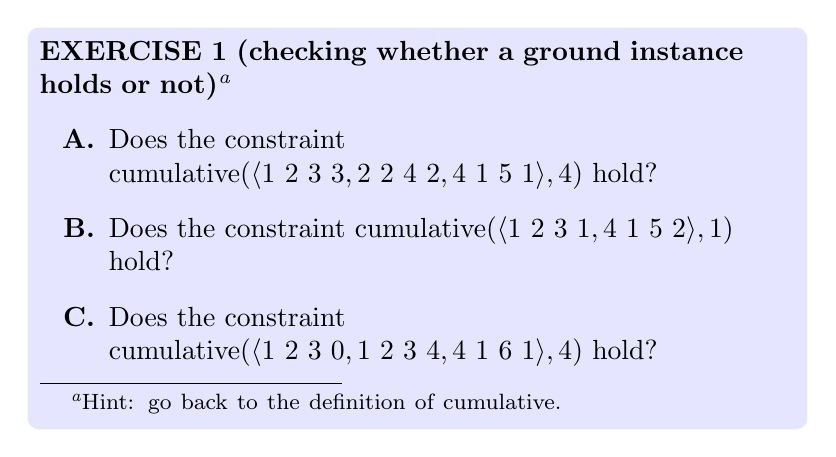
\begin{tikzpicture}
[information text/.style={rounded corners,inner sep=1ex}]
\draw
node[right,text width=9.6cm,information text,fill=blue!10]
{{\bf EXERCISE 1 (checking whether a ground instance holds or not)\footnote{Hint: go back to the definition of \ctrrefself{cumulative}.}}
\begin{enumerate}
\item
Does the constraint
\ctrrefself{cumulative}$(\langle 1~2~3~3, 2~2~4~2, 4~1~5~1\rangle, 4)$ hold?
\item
Does the constraint
\ctrrefself{cumulative}$(\langle 1~2~3~1, 4~1~5~2\rangle, 1)$ hold?
\item
Does the constraint
\ctrrefself{cumulative}$(\langle 1~2~3~0, 1~2~3~4, 4~1~6~1\rangle, 4)$ hold?
\end{enumerate}
};
\end{tikzpicture}
}
~\\

% Hint:
% reason first on the two highest tasks and then on the two smallest tasks.
{\small
\exercisecaption{\ctrrefself{cumulative}: finding all solutions}
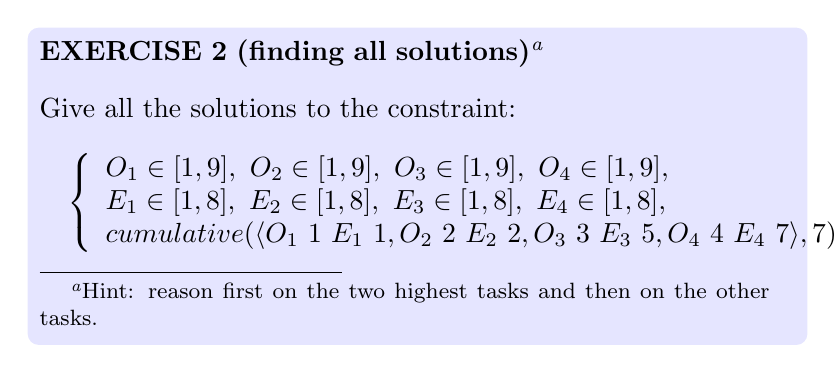
\begin{tikzpicture}
[information text/.style={rounded corners,inner sep=1ex}]
\draw[xshift=-3cm,yshift=3.3cm]
node[right,text width=9.6cm,information text,fill=blue!10]
{{\bf EXERCISE 2 (finding all solutions)\footnote{Hint: reason first on the two highest tasks and then on the other tasks.}}\\
\vspace{0.3cm}
Give all the solutions to the constraint:\\~\\
\hspace*{1em}$\left\{
\begin{array}{l}
O_1\in[1,9], ~O_2\in[1,9], ~O_3\in[1,9], ~O_4\in[1,9],\\
E_1\in[1,8], ~E_2\in[1,8], ~E_3\in[1,8], ~E_4\in[1,8],\\
\constraint{cumulative}(\langle O_1~1~E_1~1, O_2~2~E_2~2, O_3~3~E_3~5, O_4~4~E_4~7\rangle,7).\\
\end{array}
\right.$\\~\\
};
\end{tikzpicture}
}
~\\

{\small
\renewcommand\theenumi {\bf\Alph{enumi}}
\begin{tikzpicture}
[information text/.style={rounded corners,inner sep=1ex}]
\draw
node[right,text width=6cm,information text,fill=red!10]
{{\bf SOLUTION TO EXERCISE 1}\\
\begin{enumerate}
\item
\emph{No, since the first and second tasks overlap at time point $2$
and use up to $3+2$ resource units which exceeds the resource capacity $4$.}\\
\item
\emph{No, since the second task uses $2$ resource units,
while the resource capacity is $1$.}
\item
\emph{No, since for the third task the origin plus the duration is different
from the end} ($4+1\neq 6$).
\end{enumerate}
};
\begin{scope}[xshift=7.2cm,yshift=0.3cm,scale=0.30]
\draw[step=1cm,gray,very thin] (0,0) grid (5,4);
\filldraw[fill=MyRhodamine!20!white, draw=black!65, line width=0.6pt] (1,0) rectangle (3,3);
\filldraw[fill=black, draw=black] (1,0) rectangle (1.25,0.25);
\coordinate [label=left:\textcolor{MyRhodamine}{{\scriptsize$\mathbf{1}$}}] (T1) at (2.7,1.5);
\filldraw[fill=MyRedOrange!20!white, draw=black!65, line width=0.6pt] (2,3) rectangle (3,5);
\filldraw[fill=black, draw=black] (2,3) rectangle (2.25,3.25);
\filldraw[fill=MyRedOrange!20!white, draw=black!65, line width=0.6pt] (3,0) rectangle (4,2);
\coordinate [label=left:\textcolor{MyRedOrange}{{\scriptsize$\mathbf{2}$}}] (T2) at (4.15,1);
\filldraw[fill=MyPineGreen!20!white, draw=black!65, line width=0.6pt] (4,0) rectangle (5,4);
\filldraw[fill=black, draw=black] (4,0) rectangle (4.25,0.25);
\coordinate [label=left:\textcolor{MyPineGreen}{{\scriptsize$\mathbf{3}$}}] (T4) at (5.15,2.0);
\foreach \x in {1,2,3,4,5}
\draw[draw=black,line width=0.5pt] (\x,0) -- (\x,0.2);
\foreach \x in {1,2,3,4,5}
\coordinate [label=left:{\scriptsize$\x$}] (X) at (0.5+\x,-0.5);
\foreach \y in {1,2,3,4}
\draw[draw=black,line width=0.5pt] (0,\y) -- (0.2,\y);
\foreach \y in {1,2,3,4}
\coordinate [label=left:{\scriptsize$\y$}] (Y) at (-0.1,\y+0.1);
\draw[draw=red!70,line width=2.0pt] (0,4) -- (5,4);
\coordinate [label=left:{\scriptsize(A)}] (L) at (7.0,4.6);
\draw[draw=black,line width=0.8pt,->] (0,0) -- (6.75,0);
\draw[draw=black,line width=0.8pt,->] (0,0) -- (0,5.25);
\end{scope}
\begin{scope}[xshift=7.2cm,yshift=-0.9cm,scale=0.30]
\draw[step=1cm,gray,very thin] (0,0) grid (5,1);
\filldraw[fill=MyRhodamine!20!white, draw=black!65, line width=0.6pt] (1,0) rectangle (3,1);
\filldraw[fill=black, draw=black] (1,0) rectangle (1.25,0.25);
\coordinate [label=left:\textcolor{MyRhodamine}{{\scriptsize$\mathbf{1}$}}] (T1) at (2.65,0.55);
\filldraw[fill=MyRedOrange!20!white, draw=black!65, line width=0.6pt] (3,0) rectangle (4,2);
\filldraw[fill=black, draw=black] (3,0) rectangle (3.25,0.25);
\coordinate [label=left:\textcolor{MyRedOrange}{{\scriptsize$\mathbf{2}$}}] (T2) at (4.15,0.55);
\foreach \x in {1,2,3,4,5}
\draw[draw=black,line width=0.5pt] (\x,0) -- (\x,0.2);
\foreach \x in {1,2,3,4,5}
\coordinate [label=left:{\scriptsize$\x$}] (X) at (0.5+\x,-0.5);
\foreach \y in {1}
\draw[draw=black,line width=0.5pt] (0,\y) -- (0.2,\y);
\foreach \y in {1}
\coordinate [label=left:{\scriptsize$\y$}] (Y) at (-0.1,\y+0.1);
\draw[draw=red!70,line width=2.0pt] (0,1) -- (5,1);
\coordinate [label=left:{\scriptsize(B)}] (L) at (7.0,1.6);
\draw[draw=black,line width=0.8pt,->] (0,0) -- (6.75,0);
\draw[draw=black,line width=0.8pt,->] (0,0) -- (0,2.25);
\end{scope}
\end{tikzpicture}
}
~\\

{\small
\begin{tikzpicture}
[information text/.style={rounded corners,inner sep=1ex}]
\draw
node[right,text width=7.6cm,information text,fill=red!10]
{{\bf SOLUTION TO EXERCISE 2}\\
\hspace*{0.15cm}(\emph{nested disjunctions})
\begin{enumerate}
\item
\emph{Since we have a resource limit of $7$ the third task (of height $5$)
cannot overlap the fourth task (of height $7$). Since there is no slack on
the time axis (i.e., the difference between the latest end of the third and
fourth tasks and their earliest start is equal to the sum of their durations,
$8-1=3+4$), this leads to the two configurations shown on the right.}
\item
\emph{Since there is no available space on top of the fourth task,
the first and second tasks have to be put on top of the third task.
Since on top of the third task we only have a capacity of $2$
the first and second tasks cannot overlap. Since there is no
remaining slack on the time axis this leads to the two configurations
shown on the right.}
\item
\emph{Combining the two previous observations together leads to
the four solutions shown below.}
\end{enumerate}
};
\begin{scope}[xshift=8cm,yshift=1.4cm,scale=0.20]
\filldraw[fill=MyPineGreen!20!white, draw=black!65, line width=0.6pt] (1,0) rectangle (4,5);
\coordinate [label=left:\textcolor{MyPineGreen}{{\scriptsize$\mathbf{3}$}}] (T4) at (3.5,2.5);
\filldraw[fill=MyCornflowerBlue!20!white, draw=black!65, line width=0.6pt] (4,0) rectangle (8,7);
\coordinate [label=left:\textcolor{MyCornflowerBlue}{{\scriptsize$\mathbf{4}$}}] (T4) at (7.0,3.5);
\draw[draw=red!70,line width=1.0pt] (1,7) -- (8,7);
\draw[draw=red!70,line width=1.0pt] (1,0) -- (1,7);
\draw[draw=red!70,line width=1.0pt] (8,0) -- (8,7);
\end{scope}
\begin{scope}[xshift=8cm,yshift=-0.2cm,scale=0.20]
\filldraw[fill=MyPineGreen!20!white, draw=black!65, line width=0.6pt] (5,0) rectangle (8,5);
\filldraw[fill=MyCornflowerBlue!20!white, draw=black!65, line width=0.6pt] (1,0) rectangle (5,7);
\coordinate [label=left:\textcolor{MyPineGreen}{{\scriptsize$\mathbf{3}$}}] (T4) at (7.5,2.5);
\coordinate [label=left:\textcolor{MyCornflowerBlue}{{\scriptsize$\mathbf{4}$}}] (T4) at (4,3.5);
\draw[draw=red!70,line width=1.0pt] (1,7) -- (8,7);
\draw[draw=red!70,line width=1.0pt] (1,0) -- (1,7);
\draw[draw=red!70,line width=1.0pt] (8,0) -- (8,7);
\end{scope}
\begin{scope}[xshift=8.4cm,yshift=-2.1cm,scale=0.20]
\filldraw[fill=MyPineGreen!20!white, draw=black!65, line width=0.6pt] (1,0) rectangle (4,5);
\coordinate [label=left:\textcolor{MyPineGreen}{{\scriptsize$\mathbf{3}$}}] (T4) at (3.5,2.5);
\filldraw[fill=MyRhodamine!20!white, draw=black!65, line width=0.6pt] (1,5) rectangle (2,6);
\coordinate [label=left:\textcolor{MyRhodamine}{{\scriptsize$\mathbf{1}$}}] (T1) at (2.5,5.5);
\filldraw[fill=MyRedOrange!20!white, draw=black!65, line width=0.6pt] (2,5) rectangle (4,7);
\coordinate [label=left:\textcolor{MyRedOrange}{{\scriptsize$\mathbf{2}$}}] (T2) at (3.9,6);
\draw[draw=red!70,line width=1.0pt] (1,7) -- (4,7);
\draw[draw=red!70,line width=1.0pt] (1,0) -- (1,7);
\draw[draw=red!70,line width=1.0pt] (4,0) -- (4,7);
\end{scope}
\begin{scope}[xshift=8.4cm,yshift=-3.7cm,scale=0.20]
\filldraw[fill=MyPineGreen!20!white, draw=black!65, line width=0.6pt] (1,0) rectangle (4,5);
\coordinate [label=left:\textcolor{MyPineGreen}{{\scriptsize$\mathbf{3}$}}] (T4) at (3.5,2.5);
\filldraw[fill=MyRhodamine!20!white, draw=black!65, line width=0.6pt] (3,5) rectangle (4,6);
\coordinate [label=left:\textcolor{MyRhodamine}{{\scriptsize$\mathbf{1}$}}] (T1) at (4.5,5.5);
\filldraw[fill=MyRedOrange!20!white, draw=black!65, line width=0.6pt] (1,5) rectangle (3,7);
\coordinate [label=left:\textcolor{MyRedOrange}{{\scriptsize$\mathbf{2}$}}] (T2) at (3,6);
\draw[draw=red!70,line width=1.0pt] (1,7) -- (4,7);
\draw[draw=red!70,line width=1.0pt] (1,0) -- (1,7);
\draw[draw=red!70,line width=1.0pt] (4,0) -- (4,7);
\end{scope}
\begin{scope}[xshift=4.5cm,yshift=-5.7cm]
\node [single arrow, single arrow tip angle=135, single arrow head extend=1cm, draw=MyCornflowerBlue, line width=2pt,fill=MyYellowlight, single arrow, shape border rotate=270, text width=6.5cm, label=above:{{{\color{MyCornflowerBlue}\bf the four solutions}}}]
{{\tiny~~~~~~$\langle O_1 D_1 E_1 H_1, O_2 D_2 E_2 H_2, O_3 D_3 E_3 H_3, O_4 D_4 E_4 H_4\rangle$}\\
~\ding{172}~~$(\langle	{\color{MyRhodamine}\mathbf{1~1~2~1}},~~
{\color{MyRedOrange}\mathbf{2~2~4~2}},~~
{\color{MyPineGreen}\mathbf{1~3~4~5}},~~
{\color{MyCornflowerBlue}\mathbf{4~4~8~7}}\rangle)$\\
~\ding{173}~~$(\langle 	{\color{MyRhodamine}\mathbf{3~1~4~1}},~~
{\color{MyRedOrange}\mathbf{1~2~3~2}},~~
{\color{MyPineGreen}\mathbf{1~3~4~5}},~~
{\color{MyCornflowerBlue}\mathbf{4~4~8~7}}\rangle)$\\
~\ding{174}~~$(\langle	{\color{MyRhodamine}\mathbf{5~1~6~1}},~~
{\color{MyRedOrange}\mathbf{6~2~8~2}},~~
{\color{MyPineGreen}\mathbf{5~3~8~5}},~~
{\color{MyCornflowerBlue}\mathbf{1~4~5~7}}\rangle)$\\
~\ding{175}~~$(\langle	{\color{MyRhodamine}\mathbf{7~1~8~1}},~~
{\color{MyRedOrange}\mathbf{5~2~7~2}},~~
{\color{MyPineGreen}\mathbf{5~3~8~5}},~~
{\color{MyCornflowerBlue}\mathbf{1~4~5~7}}\rangle)$};
\end{scope}
\begin{scope}[xshift=0.5cm,yshift=-10.4cm,scale=0.30]
\draw[step=1cm,gray,very thin] (0,0) grid (10,7);
\filldraw[fill=MyRhodamine!20!white, draw=black!65, line width=0.6pt] (1,5) rectangle (2,6);
\filldraw[fill=black, draw=black] (1,5) rectangle (1.25,5.25);
\coordinate [label=left:\textcolor{MyRhodamine}{{\scriptsize$\mathbf{1}$}}] (T1) at (2.1,5.5);
\filldraw[fill=MyRedOrange!20!white, draw=black!65, line width=0.6pt] (2,5) rectangle (4,7);
\filldraw[fill=black, draw=black] (2,5) rectangle (2.25,5.25);
\coordinate [label=left:\textcolor{MyRedOrange}{{\scriptsize$\mathbf{2}$}}] (T2) at (3.5,6);
\filldraw[fill=MyPineGreen!20!white, draw=black!65, line width=0.6pt] (1,0) rectangle (4,5);
\filldraw[fill=black, draw=black] (1,0) rectangle (1.25,0.25);
\coordinate [label=left:\textcolor{MyPineGreen}{{\scriptsize$\mathbf{3}$}}] (T4) at (3,2.5);
\filldraw[fill=MyCornflowerBlue!20!white, draw=black!65, line width=0.6pt] (4,0) rectangle (8,7);
\filldraw[fill=black, draw=black] (4,0) rectangle (4.25,0.25);
\coordinate [label=left:\textcolor{MyCornflowerBlue}{{\scriptsize$\mathbf{4}$}}] (T4) at (6.5,3.5);
\foreach \x in {1,2,3,4,5,6,7,8,9,10}
\draw[draw=black,line width=0.5pt] (\x,0) -- (\x,0.2);
\foreach \x in {1,2,3,4,5,6,7,8}
\coordinate [label=left:{\scriptsize$\x$}] (X) at (0.5+\x,-0.5);
\foreach \y in {1,2,3,4,5,6,7}
\draw[draw=black,line width=0.5pt] (0,\y) -- (0.2,\y);
\foreach \y in {1,2,3,4,5,6,7}
\coordinate [label=left:{\scriptsize$\y$}] (Y) at (-0.1,\y+0.1);
\draw[draw=red!70,line width=2.0pt] (0,7) -- (10,7);
\coordinate [label=left:\ding{172}] (L) at (10.30,6.5);
\draw[draw=red!70,line width=1.0pt] (1,0) -- (1,7);
\draw[draw=red!70,line width=1.0pt] (8,0) -- (8,7);
\draw[draw=black,line width=0.8pt,->] (0,0) -- (10.75,0);
\draw[draw=black,line width=0.8pt,->] (0,0) -- (0,7.75);
\end{scope}
\begin{scope}[xshift=5.70cm,yshift=-10.4cm,scale=0.30]
\draw[step=1cm,gray,very thin] (0,0) grid (10,7);
\filldraw[fill=MyRhodamine!20!white, draw=black!65, line width=0.6pt] (3,5) rectangle (4,6);
\filldraw[fill=black, draw=black] (3,5) rectangle (3.25,5.25);
\coordinate [label=left:\textcolor{MyRhodamine}{{\scriptsize$\mathbf{1}$}}] (T1) at (4.1,5.5);
\filldraw[fill=MyRedOrange!20!white, draw=black!65, line width=0.6pt] (1,5) rectangle (3,7);
\filldraw[fill=black, draw=black] (1,5) rectangle (1.25,5.25);
\coordinate [label=left:\textcolor{MyRedOrange}{{\scriptsize$\mathbf{2}$}}] (T2) at (2.5,6);
\filldraw[fill=MyPineGreen!20!white, draw=black!65, line width=0.6pt] (1,0) rectangle (4,5);
\filldraw[fill=black, draw=black] (1,0) rectangle (1.25,0.25);
\coordinate [label=left:\textcolor{MyPineGreen}{{\scriptsize$\mathbf{3}$}}] (T4) at (3,2.5);
\filldraw[fill=MyCornflowerBlue!20!white, draw=black!65, line width=0.6pt] (4,0) rectangle (8,7);
\filldraw[fill=black, draw=black] (4,0) rectangle (4.25,0.25);
\coordinate [label=left:\textcolor{MyCornflowerBlue}{{\scriptsize$\mathbf{4}$}}] (T4) at (6.5,3.5);
\foreach \x in {1,2,3,4,5,6,7,8,9,10}
\draw[draw=black,line width=0.5pt] (\x,0) -- (\x,0.2);
\foreach \x in {1,2,3,4,5,6,7,8}
\coordinate [label=left:{\scriptsize$\x$}] (X) at (0.5+\x,-0.5);
\foreach \y in {1,2,3,4,5,6,7}
\draw[draw=black,line width=0.5pt] (0,\y) -- (0.2,\y);
\foreach \y in {1,2,3,4,5,6,7}
\coordinate [label=left:{\scriptsize$\y$}] (Y) at (-0.1,\y+0.1);
\draw[draw=red!70,line width=2.0pt] (0,7) -- (10,7);
\coordinate [label=left:\ding{173}] (L) at (10.30,6.5);
\draw[draw=red!70,line width=1.0pt] (1,0) -- (1,7);
\draw[draw=red!70,line width=1.0pt] (8,0) -- (8,7);
\draw[draw=black,line width=0.8pt,->] (0,0) -- (10.75,0);
\draw[draw=black,line width=0.8pt,->] (0,0) -- (0,7.75);
\end{scope}
\begin{scope}[xshift=0.5cm,yshift=-13.1cm,scale=0.30]
\draw[step=1cm,gray,very thin] (0,0) grid (10,7);
\filldraw[fill=MyRhodamine!20!white, draw=black!65, line width=0.6pt] (5,5) rectangle (6,6);
\filldraw[fill=black, draw=black] (5,5) rectangle (5.25,5.25);
\coordinate [label=left:\textcolor{MyRhodamine}{{\scriptsize$\mathbf{1}$}}] (T1) at (6.1,5.5);
\filldraw[fill=MyRedOrange!20!white, draw=black!65, line width=0.6pt] (6,5) rectangle (8,7);
\filldraw[fill=black, draw=black] (6,5) rectangle (6.25,5.25);
\coordinate [label=left:\textcolor{MyRedOrange}{{\scriptsize$\mathbf{2}$}}] (T2) at (7.5,6);
\filldraw[fill=MyPineGreen!20!white, draw=black!65, line width=0.6pt] (5,0) rectangle (8,5);
\filldraw[fill=black, draw=black] (5,0) rectangle (5.25,0.25);
\coordinate [label=left:\textcolor{MyPineGreen}{{\scriptsize$\mathbf{3}$}}] (T4) at (7,2.5);
\filldraw[fill=MyCornflowerBlue!20!white, draw=black!65, line width=0.6pt] (1,0) rectangle (5,7);
\filldraw[fill=black, draw=black] (1,0) rectangle (1.25,0.25);
\coordinate [label=left:\textcolor{MyCornflowerBlue}{{\scriptsize$\mathbf{4}$}}] (T4) at (3.5,3.5);
\foreach \x in {1,2,3,4,5,6,7,8,9,10}
\draw[draw=black,line width=0.5pt] (\x,0) -- (\x,0.2);
\foreach \x in {1,2,3,4,5,6,7,8}
\coordinate [label=left:{\scriptsize$\x$}] (X) at (0.5+\x,-0.5);
\foreach \y in {1,2,3,4,5,6,7}
\draw[draw=black,line width=0.5pt] (0,\y) -- (0.2,\y);
\foreach \y in {1,2,3,4,5,6,7}
\coordinate [label=left:{\scriptsize$\y$}] (Y) at (-0.1,\y+0.1);
\draw[draw=red!70,line width=2.0pt] (0,7) -- (10,7);
\coordinate [label=left:\ding{174}] (L) at (10.30,6.5);
\draw[draw=red!70,line width=1.0pt] (1,0) -- (1,7);
\draw[draw=red!70,line width=1.0pt] (8,0) -- (8,7);
\draw[draw=black,line width=0.8pt,->] (0,0) -- (10.75,0);
\draw[draw=black,line width=0.8pt,->] (0,0) -- (0,7.75);
\end{scope}
\begin{scope}[xshift=5.70cm,yshift=-13.1cm,scale=0.30]
\draw[step=1cm,gray,very thin] (0,0) grid (10,7);
\filldraw[fill=MyRhodamine!20!white, draw=black!65, line width=0.6pt] (7,5) rectangle (8,6);
\filldraw[fill=black, draw=black] (7,5) rectangle (7.25,5.25);
\coordinate [label=left:\textcolor{MyRhodamine}{{\scriptsize$\mathbf{1}$}}] (T1) at (8.1,5.5);
\filldraw[fill=MyRedOrange!20!white, draw=black!65, line width=0.6pt] (5,5) rectangle (7,7);
\filldraw[fill=black, draw=black] (5,5) rectangle (5.25,5.25);
\coordinate [label=left:\textcolor{MyRedOrange}{{\scriptsize$\mathbf{2}$}}] (T2) at (6.5,6);
\filldraw[fill=MyPineGreen!20!white, draw=black!65, line width=0.6pt] (5,0) rectangle (8,5);
\filldraw[fill=black, draw=black] (5,0) rectangle (5.25,0.25);
\coordinate [label=left:\textcolor{MyPineGreen}{{\scriptsize$\mathbf{3}$}}] (T4) at (7,2.5);
\filldraw[fill=MyCornflowerBlue!20!white, draw=black!65, line width=0.6pt] (1,0) rectangle (5,7);
\filldraw[fill=black, draw=black] (1,0) rectangle (1.25,0.25);
\coordinate [label=left:\textcolor{MyCornflowerBlue}{{\scriptsize$\mathbf{4}$}}] (T4) at (3.5,3.5);
\foreach \x in {1,2,3,4,5,6,7,8,9,10}
\draw[draw=black,line width=0.5pt] (\x,0) -- (\x,0.2);
\foreach \x in {1,2,3,4,5,6,7,8}
\coordinate [label=left:{\scriptsize$\x$}] (X) at (0.5+\x,-0.5);
\foreach \y in {1,2,3,4,5,6,7}
\draw[draw=black,line width=0.5pt] (0,\y) -- (0.2,\y);
\foreach \y in {1,2,3,4,5,6,7}
\coordinate [label=left:{\scriptsize$\y$}] (Y) at (-0.1,\y+0.1);
\draw[draw=red!70,line width=2.0pt] (0,7) -- (10,7);
\coordinate [label=left:\ding{175}] (L) at (10.30,6.5);
\draw[draw=red!70,line width=1.0pt] (1,0) -- (1,7);
\draw[draw=red!70,line width=1.0pt] (8,0) -- (8,7);
\draw[draw=black,line width=0.8pt,->] (0,0) -- (10.75,0);
\draw[draw=black,line width=0.8pt,->] (0,0) -- (0,7.75);
\end{scope}
\end{tikzpicture}
}
\end{ctrdesc}
